% !TEX root = ../main.tex

\chapter{基于蛋白质和药物表征学习的药物靶标对结合亲和力预测模型}

药物靶点相互作用 (DTI) 的检测是药物开发和药物重新定位的关键步骤。 在过去的几十年里,高通量筛选 (HTS) 实验大大加速了 DTI 的识别。然而,HTS 实验成本高且费时费力,无法满足探索数百万个现有药物分子化合物和数千个靶标蛋白相互作用关系的需要 \cite{n2017design, kapetanovic2008computer}。因此,我们需要建立用于自动预测 DTI 结合亲和力的计算工具 \cite{heifetz2018computational}。

目前针对药物分子-靶标蛋白结合亲和力预测的计算方法主要分为三类,即基于三维空间对接、基于相似性搜索和基于特征的方法。对于基于三维空间对接的方法,通过考虑配体的各种转换和旋转,使用靶标蛋白的三维结构来模拟结合的位置和方向,以获得不同的结合构象 \cite{ragoza2017protein, gowthaman2016darc, verdonk2003improved, paul2016mols}。 这些方法通过设计打分函数来预测有效的蛋白质-配体结合,从而最大限度地减少结合自由能。对接方法的有效性取决于蛋白质 3D 结构信息,而许多靶标蛋白质的 3D 结构仍然未知,如 GPCRs \cite{ballesteros2001g}。此外,对接过程的模拟仿真比较耗时,只能在预测规模较小的情况下使用。

基于相似性搜索的方法假设具有相似结构或理化性质的小分子化合物可以作用于具有相同或相似性质的靶标蛋白 \cite{yamanishi2008prediction, bleakley2009supervised, pahikkala2015toward, he2017simboost}。由于公共数据库中药物信息和靶点蛋白注释的迅速增加,基于相似性搜索的方法近年来得到了广泛应用。然而,它们只能用于预测与已知靶标相似的蛋白质,而无法识别新靶标蛋白的 DTI。

与基于对接和基于相似性搜索的方法不同,基于特征的方法利用从药物化合物和靶标蛋白质中提取的各种类型的特征,采用机器学习模型来预测 DTI 的关系。基于特征的方法大致可以分为两类。第一类采用协同矩阵分解技术\cite{cobanoglu2013predicting, ezzat2016drug, zheng2013collaborative}。这种方法将已知的药物-靶点关系矩阵分解为分别代表药物和靶标蛋白的两个低维特征矩阵。基于药物和靶标蛋白的特征矩阵,可以通过取特征向量的内积来获得药物和靶标蛋白的相似度矩阵。给定药物-靶点关系矩阵以及两个相似度矩阵,可以推断出潜在的 DTI 关系。例如,DTINet 通过整合各种与药物相关的信息,从异构网络 \cite{luo2017network} 中预测新的药物-靶标相互作用。 DTINet 专注于学习特征的低维向量表示,它准确地解释了异构网络中单个节点的拓扑特性,然后通过向量空间投影方案基于这些表示进行预测。第二种基于特征的方法分别使用提取的药物化合物和靶标蛋白质的特征描述符,并将 DTI 预测建模为二分类问题(是否存在相互作用)或回归问题(输出为结合亲和力的预测值)\cite{cheng2012prediction, wang2011computational, he2010predicting}。分子指纹通常用作药物子结构的描述符,而组成、转换和分布 (CTD) 通常用作蛋白质描述符。

近年来,基于特征的方法得到了更广泛的应用,因为它们对输入信息源几乎没有限制。然而,它们的性能在很大程度上依赖于特征表示。在现有的药物和靶标蛋白描述符中,分子结构信息往往缺失,从而导致预测结果不理想。由于深度神经网络 (DNN) 在图像和序列数据的自动特征学习方面取得了巨大成功,一些深度学习模型也被提出来预测药物和目标之间的结合亲和力。通过输入原始药物和靶标蛋白质数据,DNN 可以提取有用的信息进行预测。例如,DeepDTA 采用卷积神经网络 (CNN) 提取局部序列模式作为药物-靶标结合亲和力预测的高级特征表示 \cite{ozturk2018deepdta}。另一种称为 DeepConv-DTI \cite{lee2019deepconv} 的方法也采用了 CNN。与主要关注蛋白激酶的 DeepDTA 不同,DeepConv-DTI 是在具有不同类型蛋白质的更大规模数据集上训练的。后来,提出了一个名为 GraphDTA \cite{nguyen2019graphdta} 的 DTI 模型来预测药物-靶标结合亲和力,这是一种用于激酶型靶标蛋白最先进的方法。尽管上述方法取得了进展,但仍有很大的空间可以改进药物和靶蛋白的特征表示以增强 DTI 的预测。

本章将详细介绍我们提出的 EmbedDTI 模型,基于靶标蛋白质序列和药物分子序列的表征学习进行药物分子-靶标蛋白结合亲和力的预测。本章主要分为七个部分展开,分别是:实验数据集构建、EmbedDTI介绍、初始特征提取、基于深度学习的特征训练、结合亲和力预测、实验结果和EmbedDTI 模型注意力机制的可视化解释。

\section{实验数据集构建}

\subsection{结合亲和力指标}
结合亲和力提供了有关药物-靶标蛋白对(DT)之间相互作用的特定信息。它可以通过半数最大抑制浓度($IC_{50}$)、解离常数($K_d$)、抑制常数($K_i$)和结合常数($K_a$)等指标来衡量)。 $IC_{50}$代表抑制一半指定生物过程(或过程中的成分,如酶、受体、细胞等)所需的药物或抑制剂的浓度。 $K_i$ 反映了抑制剂对靶标蛋白的抑制强度。该值越小,抑制能力越强。 $K_d$ 反映了药物化合物对靶标蛋白的亲和力。该值越小,结合亲和力越强。在某些情况下,它相当于 $K_i$。 $K_a$ 是 $K_d$ 的倒数。因此,$K_a$ 的值越大,结合亲和力越强。遵循先前研究 \cite{he2017simboost} 的做法,我们采用对数转换的 $K_d$(方程(\ref{eq:1}))作为模型输出。

\begin{equation}
  pK_d = - \log_{10}{(\frac{K_d}{1e9})}
\label{eq:1}
\end{equation}

\subsection{实验数据集}
我们在两个基准集上评估我们的模型,Kinase 数据集 Davis \cite{davis2011comprehensive} 和 KIBA 数据集 \cite{tang2014making},它们被用于 DeepDTA \cite{ozturk2018deepdta}、WideDTA \cite{ozturk2019widedta}、PADME \cite{feng2018padme}、MT-DTI \cite{shin2019self} 和 GraphDTA \cite{nguyen2019graphdta}模型。表 \ref{table:dti_datasets} 显示了这两个数据集的概述。

\begin{table}[!htbp]
\centering
\bicaption[Davis 和 KIBA 数据集]{Davis 和 KIBA 数据集。}{Datasets of Davis and KIBA.}
\caption{Davis 和 KIBA 数据集}
\scalebox{1.2}{
\begin{tabular}{c|c|c|c}
\toprule
数据集 & 药物分子数量 & 靶标蛋白数量 & DT数量 \\
\midrule
Davis & 68 & 442 & 30056\\
\hline
KIBA & 2111 & 229 & 118254 \\
\bottomrule
\end{tabular}}
\label{table:dti_datasets}
\end{table}

\section{EmbedDTI 模型介绍} \label{5.2}
本文中,我们通过预测药物分子-靶标蛋白对之间的结合亲和力,将 DTI 问题视为一个回归任务,并提出了一种称为 EmbedDTI 的深度学习模型如图\ref{fig:EmbedDTI}所示。

\begin{figure}[!htbp] 
\centering
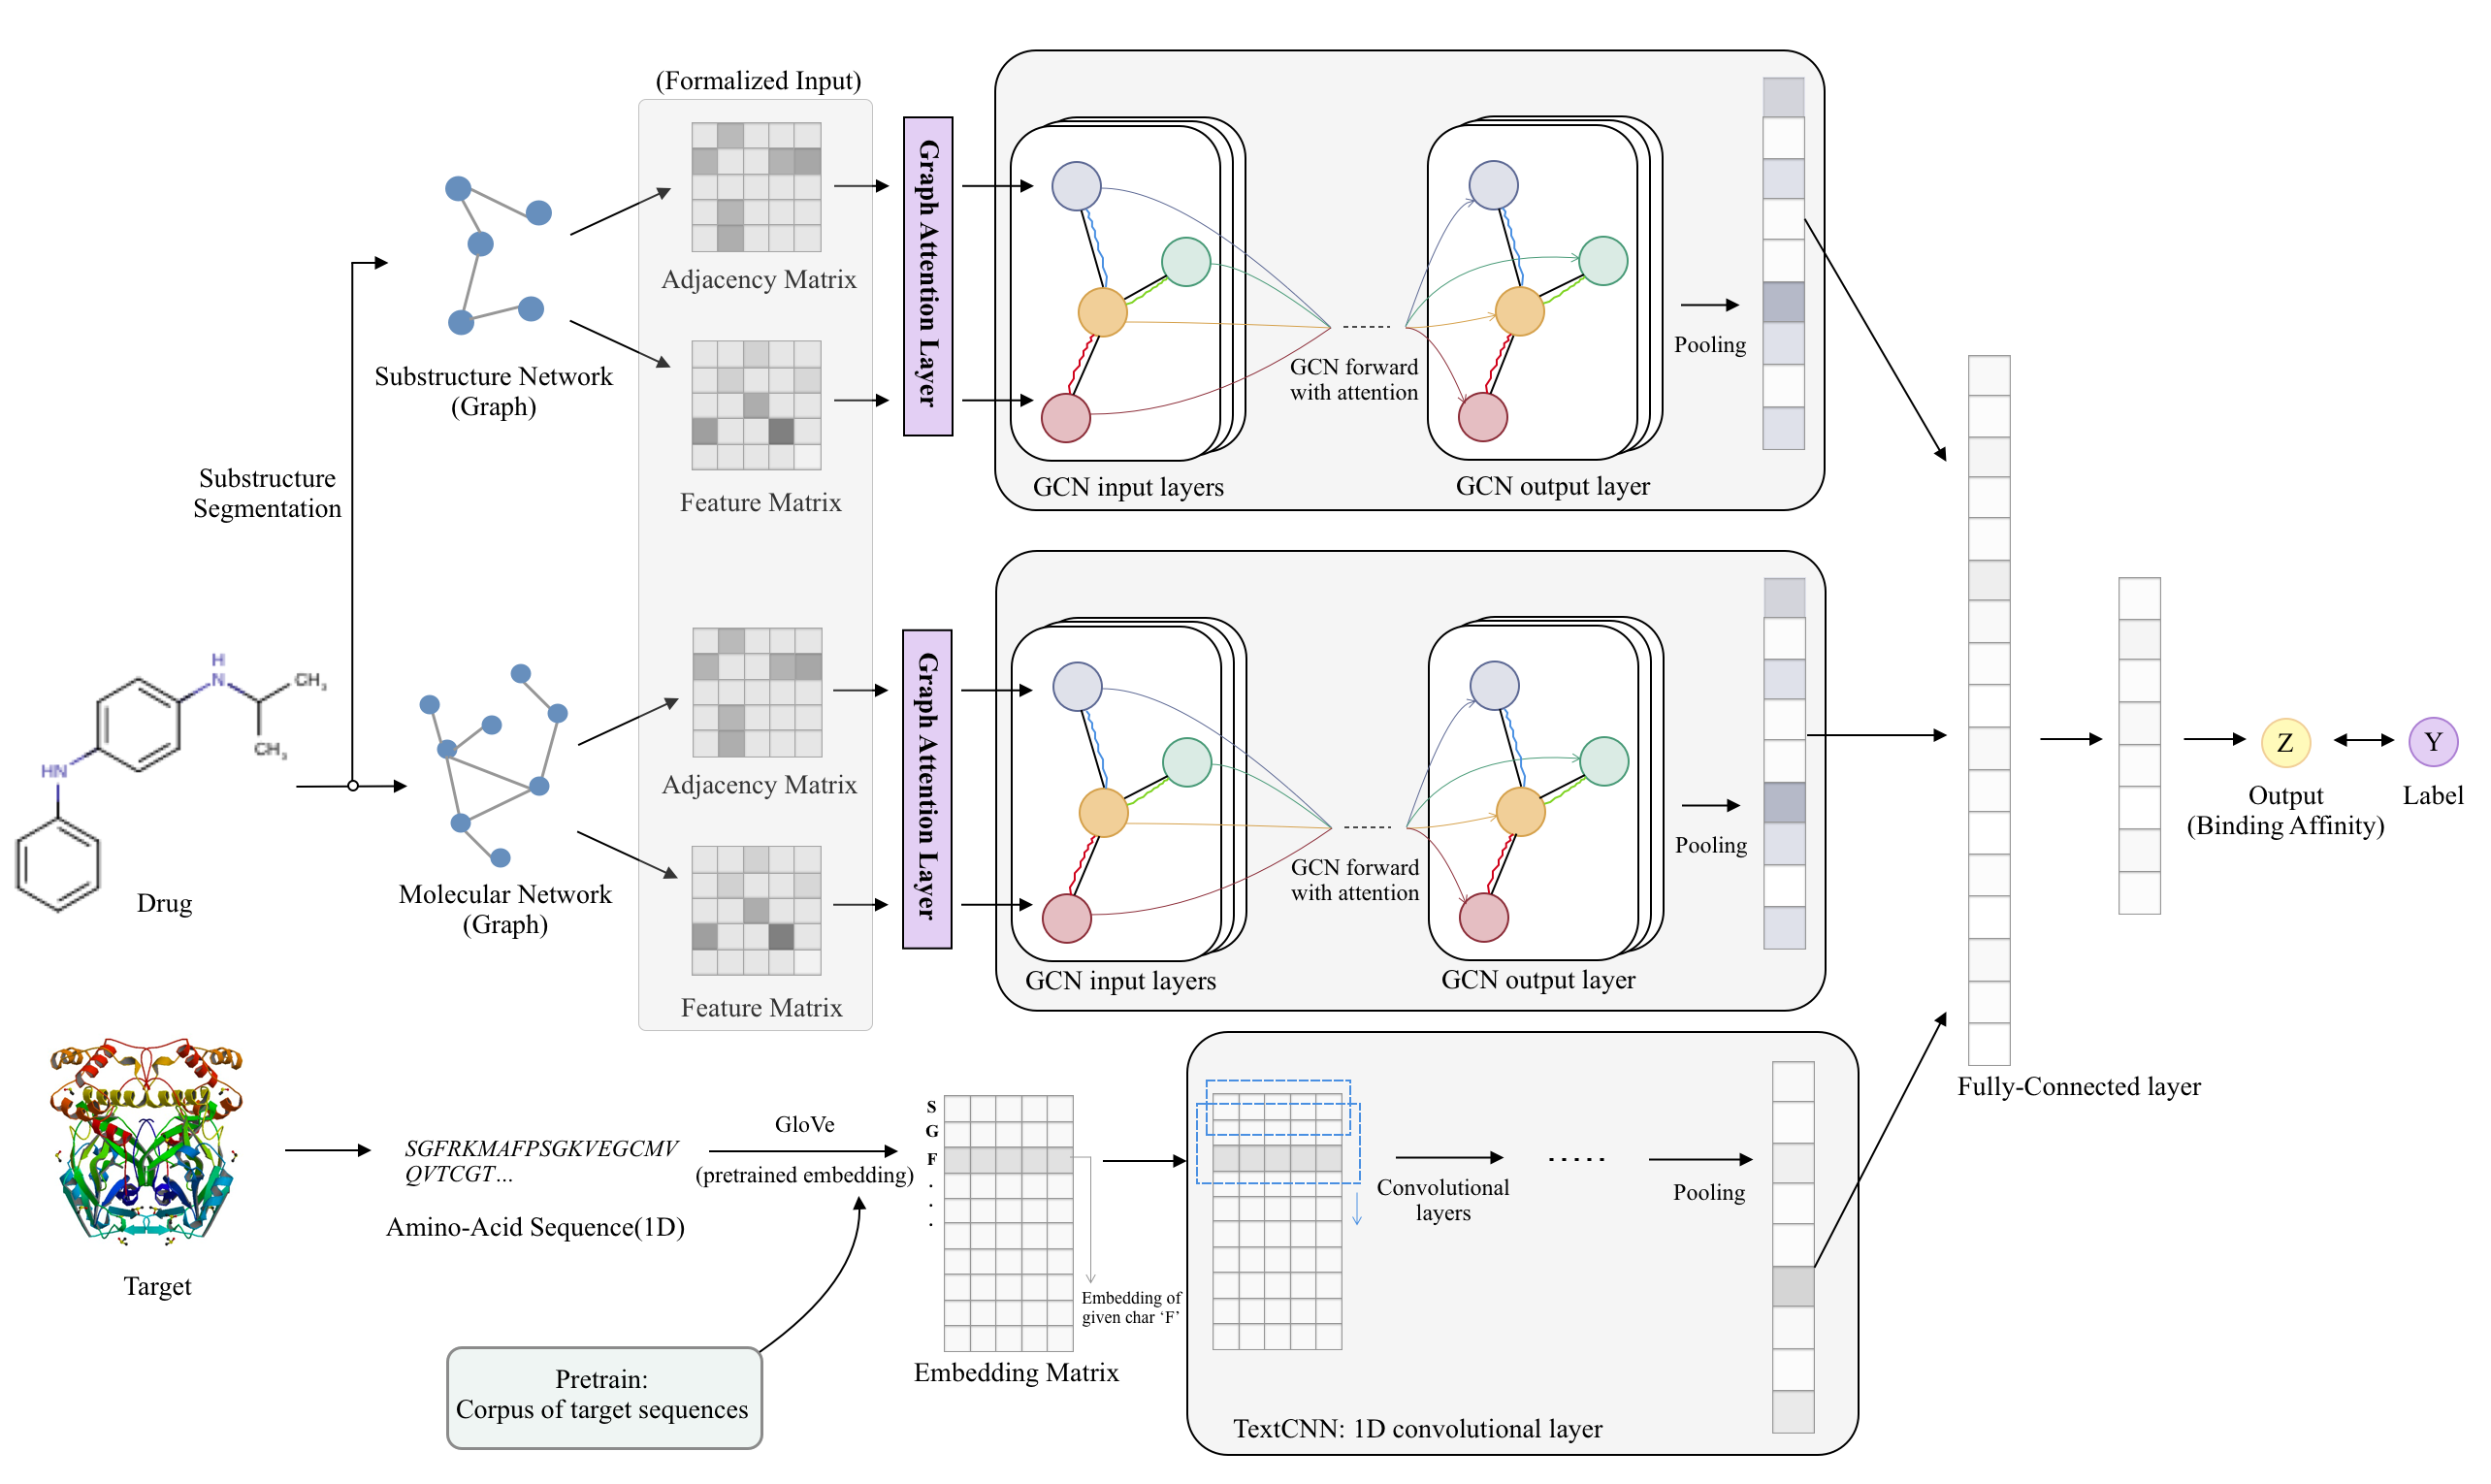
\includegraphics[width=1\textwidth]  {imgs/model.png}
\bicaption[EmbedDTI 模型结构]
        {EmbedDTI 的模型结构。对于蛋白质序列,我们利用 GloVe 方法对氨基酸的初始特征嵌入进行预训练,并将它们提供给 CNN 模型进行表征学习。对于药物分子,我们构建了两个层次的图来表示复合结构信息,即原子图和子结构图。不同级别的图分别通过注意力机制和几个 GCN 层得到特征嵌入表示向量。将三个嵌入向量连接起来,通过几个全连接层输出得到药物-靶标对的结合亲和力预测值。}
        {Model architecture of EmbedDTI. For protein sequences, we leverage GloVe for pretraining the feature embeddings of amino acids and feed them to a CNN model for representation learning. For~drugs, we construct two levels of graphs to represent compound structural information, namely the atom graph and substructure graph. Graphs of different levels provide an embedding representation vector respectively through attention and several GCNs. Three embedding vectors are concatenated to output the binding affinity of the drug-target pairs through several fully connected layers.}
\label{fig:EmbedDTI}
\end{figure}

EmbedDTI 模型主要由三个部分组成,分别是:初始特征提取、基于深度学习的特征训练和结合亲和力预测。EmbedDTI 模型的原始输入是靶标蛋白质的氨基酸序列和药物分子化合物的 SMILES 序列。在初始特征提取部分,我们使用 GloVe 算法 \cite{pennington2014glove} 来获得预训练好的氨基酸嵌入表征。对于药物分子,我们将 SMILES 序列转换为两个图数据结构,以保留尽可能多的化学结构信息用于药物分子序列表征学习。其中一个是基于原子的药物分子结构图,它由作为节点的原子和作为边的原子之间的化学键组成,表示单个原子及其相关邻居节点的信息。另一个是基于子结构图的药物分子结构图,即每个节点表示化合物中的子结构而不是原子,每条边表示子结构直接的连接关系。根据每一个图结构,我们得到其邻接矩阵。对于图中的每个节点,我们通过提取一些化学和数据结构方面的特征,从而形成一个特征矩阵。

在特征学习部分,对于靶标蛋白质,我们将预训练的氨基酸嵌入表征向量输入到 TextCNN 网络中以获得高级的蛋白质序列特征抽象表示。经过多层卷积操作和最大池化层后,我们获得了每个蛋白质序列的嵌入表征向量。由于药物分子化合物包含重要的结构信息、物理和化学性质,简单的CNN卷积运算会忽略了大量的结构和化学背景知识。因此,我们将化合物表示为图数据结构,以广泛保留序列中的领域知识。
对于每种药物,我们将从基于原子的药物分子结构图和基于子结构的药物分子结构图中获得两个邻接矩阵和特征矩阵分别送入 GCN 网络进行训练。最大池化层用于聚合每个节点的特征以获得整个图的嵌入表征向量。此外,我们在基于原子和基于子结构分支的 GCN 网络之前添加了一个点积的注意力机制层,以帮助了解每个节点(原子或子结构)在图中的相对重要性。

特征表征学习后,我们将蛋白质序列的嵌入表征向量、基于原子的药物分子结构图的嵌入表征向量、基于子结构的药物分子结构图的嵌入表征向量拼接为一个完整的向量,并将其送到几个全连接层中,以获得药物分子-靶标蛋白对的结合亲和力分数。

以下\ref{5.3}-\ref{5.5}节描述了模型三个部分的详细信息。


\section{初始特征提取} \label{5.3}
\subsection{蛋白质序列的初始特征提取}
在 DTI 任务中,我们使用靶标蛋白质序列作为模型的输入。每条蛋白质序列由20多种氨基酸排列组合而成。 EmbedDTI 模型中,蛋白质序列的初始输入特征是从氨基酸序列中提取的。 为了获得氨基酸序列的良好表示,我们利用自然语言处理中的词嵌入技术对大型蛋白质数据库 UniRef50 进行预训练,并获得氨基酸的嵌入表征向量。 UniProt 的参考簇 UniRef 提供来自 UniProt 知识库(包括同种型)和选定的 UniParc 记录的序列聚类集,以便在多个分辨率下获得序列空间的完整覆盖,同时隐藏冗余序列(但不是它们的描述信息)。与 UniParc 不同的是,UniRef 中的序列片段是合并的:UniRef100 数据库将来自任何生物体的具有 11 个或更多残基的相同序列和子片段合并到一个 UniRef 条目中,显示代表性蛋白质的序列、所有合并的登录号条目和链接到相应的 UniProtKB 和 UniParc 记录。 UniRef90 是通过使用 MMseqs2 算法 \cite{steinegger2017mmseqs2} 对具有 11 个或更多残基的 UniRef100 序列进行聚类而构建的,这样每个聚类都由具有至少 90\% 的序列同一性和 80\% 与集群的最长序列(又名种子序列)重叠的序列构建的。类似地,UniRef50 是通过对 UniRef90 种子序列进行聚类而构建的,这些种子序列与簇中最长的序列具有至少 50\% 的序列同一性和 80\% 的重叠。UniRef90 和 UniRef50 分别使数据库大小减少了大约 58\% 和 79\%,从而提供了更快的序列相似性搜索。我们使用 UniRef50 数据库(https://www.uniprot.org/)作为预训练的语料库,包括 48,524,161 条氨基酸序列。

我们使用 GloVe \cite{pennington2014glove} 词嵌入模型用于获得氨基酸的初始特征嵌入表示。我们将每个氨基酸视为蛋白质序列中的一个单词对其进行预训练学习。

\subsection{药物分子序列的图结构表示}
SMILES(Simplified molecular input line entry specification)\cite{weininger1988smiles},即简化分子线性输入规范,是一种用 ASCII 字符串明确描述分子结构的规范。SMILES 序列是药物分子的线形表示符号,用于用单行文本表达化合物的结构,可以表示药物分子的原子类型以及原子之间的连接关系等信息。由于 SMILES 用一串字符来描述一个二维化学结构,它必然要将化学结构转化成一个生成树,它采用纵向优先遍历树算法。转化时,先去掉氢,再把环打开。表示时,被拆掉的键端的原子用数字标记,支链写在小括号里。上述过程如图 \ref{fig:SMILES} 所示。通过开源化学信息软件 RDKit 可以将药物分子 SMILES 序列转化为药物分子的结构图。


\begin{figure}[!htbp] 
\centering
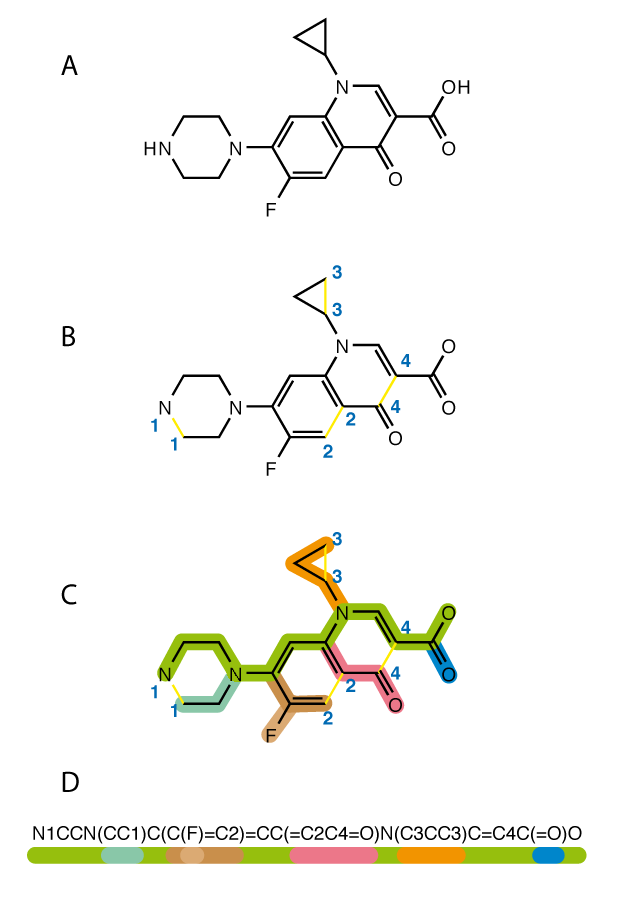
\includegraphics[width=0.8\textwidth]  {imgs/SMILES.png}
\bicaption[SMILES 序列 \cite{weininger1988smiles}图示]{SMILES 序列 \cite{weininger1988smiles}图示。}
{Process of SMILES sequences.}
\label{fig:SMILES}
\end{figure}

对于药物分子的 SMILES 序列,我们将其表示为基于原子的药物原子结构图和基于子结构的药物子结构结构图。药物分子的原子结构图可以通过从 SMILES 字符串转换得到。药物分子化合物在计算机中通常表示为图形结构的数据,其中图形的顶点和边分别对应于原子和化学键,这与药物分子的原子结构图相符。通过开源化学信息软件 RDKit 提供的函数可以将药物分子 SMILES 序列转化为药物分子的原子结构图,并为图中的每一个原子进行编号。

药物分子的原子结构图可以表示短距离原子之间的结构信息,但是忽略了分子化合物中的子结构,这些子结构在决定化合物的性质和反应中起着重要作用。例如,苯环中的单个原子可以了解其相邻原子的信息,但很难从整体上了解整个苯环的结构以及其在药物分子中发挥的作用。因此,我们定义了子结构,并将原始的基于原子的药物原子结构图转换为更高级别的药物子结构结构图,其中药物子结构结构图中的节点和边分别对应于子结构和子结构之间的连接。

药物分子的原子结构图的一个主要限制是它平等对待所有的边并从单个顶点提取信息,然而原子和它相关边通常成对发挥作用。以图 \ref{fig:invalid} 为例,蓝色原子表示的化学键对整个分子很重要,因此,药物分子中独立的化学键对整个分子的结构和化学性质起着关键作用。然而如果从苯环子结构(绿色环)中分离出来,红色原子表示的化学键在结构和化学性质上是没有意义的。因此,我们提出了一种分割药物分子的方法,从而获得了完整的药物子结构集合,以确保数据库中的所有化合物都可以由集合中的子结构组成。

\begin{figure}[!htbp] 
\centering
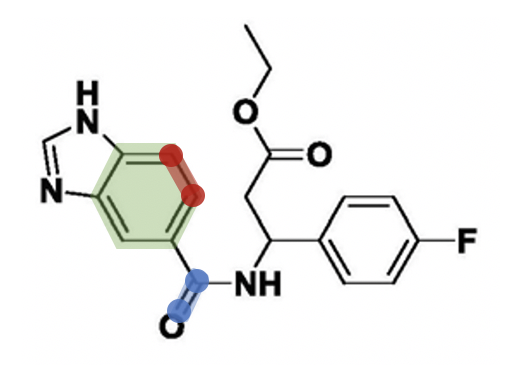
\includegraphics[width=0.7\textwidth]  {imgs/invalid.png}
\bicaption[分子中不同化学键在原子结构图中的不同作用]{分子中不同化学键在原子结构图中的不同作用。两种不同类型的化学键,红色标记的键是环中的键,而蓝色标记的键是任何环外的键。}
{Different chemical bonds in the molecule play different roles in the atomic structure diagram. There are two different types of chemical bonds, the bonds marked in red are the bonds in the ring, and the bonds marked in blue are any bonds outside the ring.}
\label{fig:invalid}
\end{figure}

如图 \ref{fig:split_diagram} 所示,我们将整个药物分子切割成子结构。子结构由一个环状子结构或者由不属于环的化学键连接的一对原子组成。这样,药物分子化合物就可以看成是由子结构连接起来的拓扑图。子结构切割算法在算法 \ref{alg:1} 中制定,其中药物分子对象通过 RDKit 中的 Chem.MolFromSmiles 函数获得。$V_1$ 和 $V_2$ 分别表示药物中独立的化学键和简单环。化学键是从 GetBonds 函数中提取的,而简单环是从 Chem.GetSymmSSSR 函数中提取的。最后,我们得到了一个不在任何环中的化学键以及与其他环共享的原子少于 3 个的独立环的子结构词汇表集合。

\begin{figure}[!htbp] 
\centering
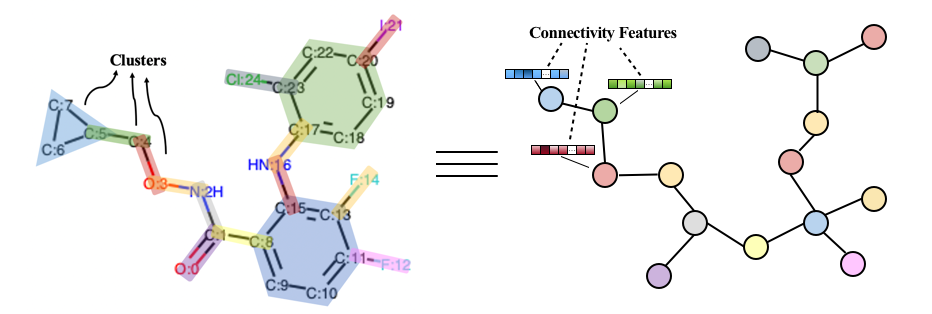
\includegraphics[width=1\textwidth]  {imgs/split_diagram.png}
\bicaption[药物子结构分割示例]{药物子结构分割示例。左边的图是药物的原子级结构图,其中子结构用不同的颜色标记。右边的是药物的子结构级图,其中每个子结构由图中的单个节点表示。}
{Example of drug substructure segmentation. The figure on the left is a diagram of the atomic structure of the drug, where the substructures are marked with different colors. On the right is a substructure level diagram of the drug, where each substructure is represented by a single node in the graph.}
\label{fig:split_diagram}
\end{figure}

% \begin{algorithm}[!htbp]
% \bicaption[药物分子 $G = (V, E)$ 子结构分割算法]{药物分子 $G = (V, E)$ 子结构分割算法}{Drug molecule $G = (V, E)$ substructure segmentation algorithm}
% \label{alg:1}
% \hspace*{0.02in} {\bf 输入:} 
% 化合物分子的 SMILES 序列 \\
% \hspace*{0.02in} {\bf 输出:} 
% 药物分子的子结构集合 $C$
% \begin{algorithmic}
% % \Require $n \geq 0$
% % \Ensure $y = x^n$
% \State 获得 SMILES 序列的药物分子对象
% \State 给化合物分子中的原子编号
% \State 初始化:药物分子的子结构集合 $C = \varnothing$
% \State 构建 $V_1$ $\gets$ 化合物分子中边 $\in E$ 的集合
% \State 构建 $V_2$ $\gets$ 化合物分子$G$ 中简单环的集合
% \For{在 $V_1$ 中的每条边 $e_i$}
% 	\If{$e_i$ 不属于任何一个简单环} 
% 		\State 将 $e_i$ 添加到药物分子的子结构集合 $C$ 的词汇表中
% 	\EndIf
% \EndFor
% \For{在 $V_2$ 中的每一个环$r_i$} 
%     \For{在$V_2$中的每一个环$r_j$,其中$i \neq j$}
%         \State $inter = r_i \cap r_j$
%         \If{ $inter$ 的长度 $\geq$ 3}
%             \State $tmp$ $\gets$ 将 $r_1,r_2$ 合并为一个独立的环
%             \State $r_i$ $\gets$ $tmp$
%             \State $r_j$ $\gets$ $tmp$
%         \EndIf
%     \EndFor
% \EndFor
% \State 从 $V_2$ 中删除重复的药物分子子结构
% \State 将 $V_2$ 中的每个子结构添加到药物分子的子结构集合 $C$中
% \State \Return 药物分子的子结构集合 $C$
% \end{algorithmic}
% \end{algorithm}

算法环境可以使用 \pkg{algorithms} 宏包或者较新的 \pkg{algorithm2e} 实现。
算法~\ref{algo:algorithm} 是一个使用 \pkg{algorithm2e} 的例子。关于排版算法环境
的具体方法,请阅读相关宏包的官方文档。

\begin{algorithm}[!htbp]
  \caption{算法示例}
  \label{alg:1}
  \small
  \SetAlgoLined
  \KwData{this text}
  \KwResult{how to write algorithm with \LaTeXe }

  initialization\;
  \While{not at end of this document}{
    read current\;
    \eIf{understand}{
      go to next section\;
      current section becomes this one\;
    }{
      go back to the beginning of current section\;
    }
  }
\end{algorithm}

\subsection{药物分子序列的初始特征提取} \label{5.3.3}
对于药物原子级结构图 $G=(V,E)$ ,其中 $V$ 是图中所有节点(药物分子中的原子)的集合,$E$ 是图中所有边(药物分子中的化学键)的集合。每一个节点 $i$ 都有其特征 $x_i$,所有的节点特征 $x_i$ 构成了一个特征矩阵 $X_atom \in \mathbb{R}^{N \times d}$ ,其中 $N$ 表示节点数,$d$ 表示每一个节点的特征数,即每一个节点特征向量的维数。我们利用开源化学信息软件 RDKit 提取每一个原子节点的初始特征。将每个原子节点的初始特征表示为一个 one-hot 特征向量,包含八种信息(原子符号、原子在药物分子中的度数、原子所连接的显式和隐式氢原子总数、 隐式连接的氢原子数,显式和隐式原子的总价数,原子的电荷数,原子是否属于芳香族,以及原子是否在环中),从而为每个原子节点得到一个 101 维的 one-hot 初始特征向量表示。 

和药物原子级结构图提取原子节点的初始特征向量表示类似,对于药物子结构级结构图我们提取每一个子结构节点的初始特征。将每个子结构节点特征表示为一个 one-hot 特征向量,包含基于图论的五种信息(原子数,和其他子结构连接的边数,显式和隐式的氢原子数,是否含有环,是否含有不属于简单环的化学键),从而为每个子结构节点得到一个 35 维的 one-hot 向量初始特征表示。

\section{基于深度学习的特征训练}
\subsection{TextCNN 模型介绍}
extCNN \cite{chen2015convolutional} 是由 Kim 于 2014 年提出的基于文本的卷积神经网络,主要用于句子分类任务,例如情感分析和问题分类等。TextCNN 是基于卷积神经网络(CNN)的序列化处理模型。

CNN 模型主要由卷积层和应用于输出层的非线性激活函数所组成,它的卷积层不同于其他神经网络。为了完成图像分类任务,CNN 会遍历像素矩阵的每个角、向量和维度。卷积层通常由多个特征组成,例如检测边缘、角点和纹理等。卷积层通过在像素矩阵上滑动可以检测所有的特征。

在 TextCNN 中,输入是一段文本,可以将文本视为时序数据。假设文本分词后有 $S$ 个单词,对于每一个单词,词嵌入向量为 $D$ 维,因此对于这段文本,可以得到一个 $A \in \mathbb{R}^{S*D}$ 的词嵌入矩阵。在 CNN 中,过滤器可以上下左右滑动,但是在文本中有所不同,因为针对单词的词向量层次左右滑动是没有意义的,因此过滤器采用上下滑动的方式获取不同宽度的视野。假设有一个宽度为 $D$,高度为 $h$ 的卷积核矩阵 $w$,对于词嵌入矩阵 $A$ 进行卷积操作可以表示为:

\begin{equation}
  o_i = w \cdot A[i:i+h-1], i = 1,2,...,s-h+1
\end{equation}
其中$A[i:j]$表示矩阵$A$的第$i$行到第$j$行。

加上偏置$b$,使用激活函数$f(x)$激活后,得到如下特征:

\begin{equation}
  c_i = f(o_i + b)
\end{equation}

由于不同尺寸的卷积核得到的特征大小是不同的,因此对于所有的卷积特征使用最大池化操作,将池化后的值拼接起来得到最终的特征向量,最终将这个特征向量输入 softmax 层进行分类。

TextCNN 的网络结构简单,可以利用不同大小的卷积核提取文本中的关键信息,从而能够更好的捕捉到文本的局部相关性。

\subsection{基于 TextCNN 的蛋白质特征学习}
如前所述,我们使用 GloVe 模型获得每个氨基酸的预训练词嵌入向量 $e_i$ ($0 \leq i \leq L$,其中 $L$ 代表靶标蛋白质序列的最大长度),然后我们将由氨基酸的词嵌入向量构成的词嵌入矩阵 $E$ 送入 TextCNN 网络中用于进一步的特征学习。 我们采用三层的 TextCNN 模型,通过在氨基酸序列附近操作的卷积核提取局部的序列特征。 TextCNN 后面接两个全连接层,为每个靶标蛋白质序列生成一个 128 维的表示向量 $P$。

\subsection{GCN 模型介绍}
传统的数据,例如图片和语言等,是属于欧几里得空间的数据,它们是比较规则的,具有维度的概念。我们可以使用 CNN、RNN、LSTM 等深度神经网络处理这类的数据。然而,现实生活中的数据不全是这种数据,有很多不规则的数据结构,例如药物分子化合物、社交网络等典型的图数据结构,这类数据可以视为具有无限维度,缺少了图片数据的平移不变性,很难用 CNN、RNN 等神经网络进行学习。因此,2017 年 Tomas 等人提出了图卷积神经网络(GCN)模型 \cite{kipf2016semi}, 主要用于解决非欧几里得空间的图数据。和 CNN 的思想类似,GCN 也采用了一种特征提取的方法,可以使用这些特征实现图节点分类、链接检测、聚类分析等任务。

GCN 是频域卷积方法的一阶局部近似,其由多个卷积层组成,每一个卷积层对节点一阶邻域的信息进行聚合生成新的节点表示,通过多个卷积层的传播可以实现多阶邻域信息的传递,从而达到 CNN 中感受野的效果。对于图 $G=(V,E)$,其中 $V$ 是图中节点的集合,$E$ 是图中边的集合。每一个节点都有其对应的特征 $x_i$。假设使用矩阵 $X \in \mathbb{R}^{N\times d}$ 表示所有节点的特征矩阵,其中 $N$ 代表图中的节点数,$d$ 代表每个节点的特征数量,即特征向量的维数。节点的连接边关系形成了一个$N\times N$维的邻接矩阵 $A$。将 $X \in \mathbb{R}^{N\times d}$ 和 $A \in \mathbb{R}^{N\times N}$ 作为 GCN 层的输入。GCN层与层之间的信息传播可以用如下公式表示:

\begin{equation}
  H^{(l+1)} = \sigma(\tilde{D}^{-\frac{1}{2}}\tilde{A}\tilde{D}^{-\frac{1}{2}}H^{(l)}W^{(l)})
\end{equation}
其中 $\tilde{A}$ 是邻接矩阵 $A$ 加上自连接边得到的矩阵,$\tilde{D}$是 $\tilde{A}$ 的度矩阵(一个对角阵,对角元素为和各个顶点相关联的边的数量),$H^{(l)}$ 表示多层图卷积层的第 $l$ 层的特征矩阵。$\sigma$ 是一个激活函数,比如ReLU。对于输入层,特征矩阵 $H^{(0)}$ 等于 $X$。经过多层图卷积操作后,得到 GCN 模型节点的输出嵌入表示为 $Z \in \mathbb{R}^{N\times F}$,其中 $F$ 表示过滤器的数量。为了获得整个图数据结构的嵌入表征,在多层图卷积层之后连接一个最大池化层,和传统 CNN 模型中的池化操作类似,最大池化操作是对图结构的一个合理缩小。

由于药物分子结构是一种不规则的图数据结构,因此非常适合使用 GCN 来学习药物分子结构的嵌入表示,通过邻域节点信息的传播与聚合,可以获得节点的局部相关特征,进而可以捕捉到图的全局信息。

\subsection{基于 GCN 的药物分子特征学习}
对于原子级的药物分子结构图,我们将上一节 \ref{5.3.3} 中得到的原子级图的邻接矩阵 $A_{atom}$ 和初始特征矩阵 $X_{atom}$ 输入三层的 GCN 网络中,提取原子级图中每一个原子的嵌入特征表示。然后经过最大池化操作,得到原子级药物分子的表征向量 $A_m$。对于子结构级的药物分子结构图,我们将上一节 \ref{5.3.3} 中得到的子结构级的邻接矩阵 $A_{sub}$ 和初始特征矩阵 $X_{sub}$ 输入三层的 GCN 网络中,提取子结构级图中每一个子结构的嵌入特征表示。经过最大池化操作,得到子结构级药物分子的表征向量 $C_q$ 。图 \ref{fig:gcn} 以原子级的药物分子结构图为例,展示了 GCN 的特征学习过程。


\begin{figure}[!htbp] 
\centering
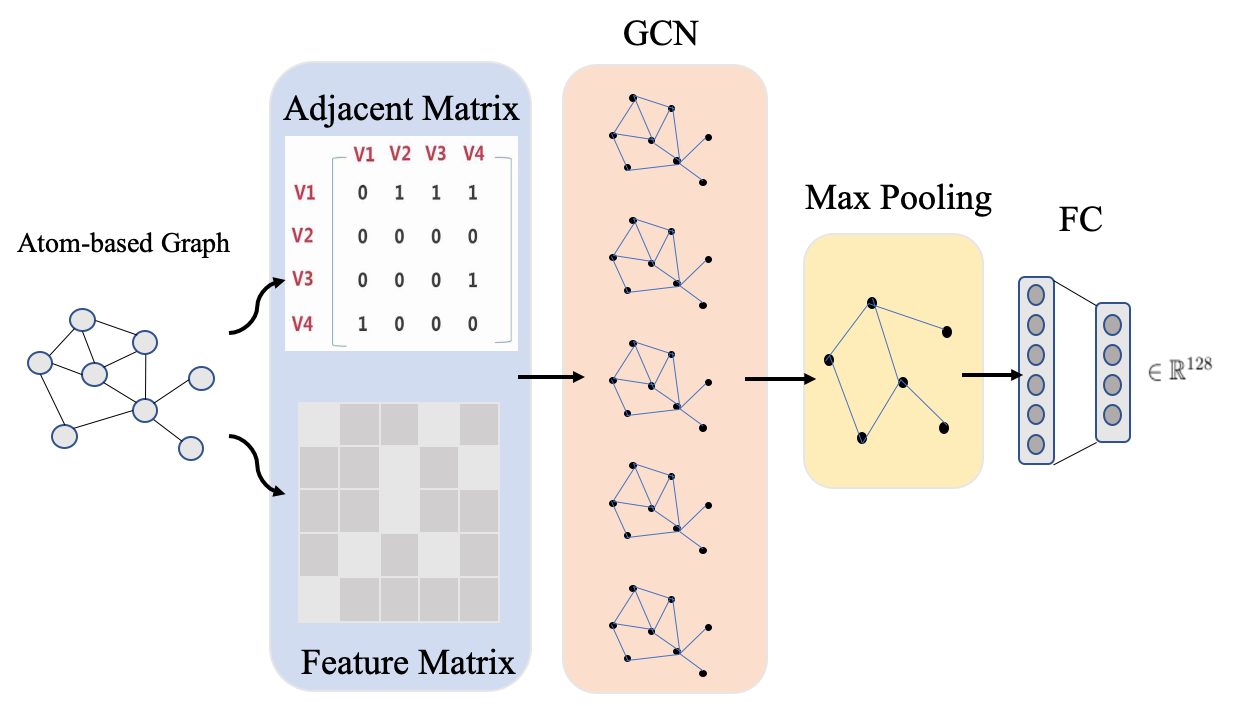
\includegraphics[width=1\textwidth]  {imgs/gcn.png}
\bicaption[GCN 对图的特征学习过程]{GCN 对图的特征学习过程。以图的邻接矩阵和特征矩阵作为输入,经过卷积运算得到节点级表示。然后,将节点级表示通过最大池化层以获得图级表示。最后对图级表示矩阵进行扩展,通过几个全连接层得到一个128维的向量。}
{GCN's feature learning process for graphs. Taking the adjacency matrix and feature matrix of the graph as input, the node-level representation is obtained through convolution operation. Then, the node-level representation is passed through the maximum pooling layer to obtain the graph-level representation. Finally, the graph-level representation matrix is expanded, and a 128-dimensional vector is obtained through several fully connected layers.}
\label{fig:gcn}
\end{figure}

此外,在 GCN 的卷积操作之前,我们添加了一个基于点积的注意力层来帮助学习每个节点(原子或子结构)的相对重要性。此时,$H^{(0)}$ 如方程(\ref{eq:2})所示。 图 \ref{fig:gcn_forward} 说明了这个注意力机制的前向传播过程。

\begin{equation}
  H^{(0)} = W \times X,
\label{eq:2}
\end{equation}
其中,$W$表示注意力权重矩阵。

\begin{figure}[!htbp] 
\centering
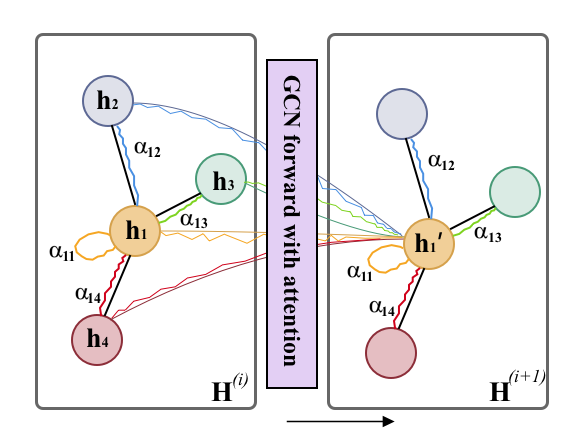
\includegraphics[width=0.85\textwidth]  {imgs/gcn_forward.png}
\bicaption[增加注意力机制的 GCN 前向传播过程]{增加注意力机制的 GCN 前向传播过程。注意力模块会考虑每一对节点 $i$ 和 $j$,并为它们分配注意力权重 $\alpha_{ij}$,表示节点 $j$ 在传播过程中对节点 $i$ 具有 $\alpha_{ij}$ 加权的影响。}
{GCN forward layer with attention. The~attention module will consider each pair of nodes and assign them with attention weight $\alpha_{ij}$, which indicates the node $j$ has $\alpha_{ij}$-weighted influence on node $i$ during the~propagation.}
\label{fig:gcn_forward}
\end{figure}


\section{结合亲和力预测} \label{5.5}
经过特征学习,我们得到了三个128维的特征向量 $P$、$A_m$ 和 $C_q$,分别是靶标蛋白、原子级药物分子和子结构级药物分子的表征向量。我们将它们拼接成一个特征嵌入向量 $T$ (方程(\ref{eq:3})) 并将它传递到三个全连接层中以获得药物分子-靶标蛋白对的结合亲和力分数。

\begin{equation}
    T = P \oplus A_{m} \oplus C_{q} \in \mathbb{R}^{384}
\label{eq:3}
\end{equation}

\section{实验结果}
\subsection{实验设置}
我们评估了 EmbedDTI 在两个基准集 Davis 数据集和 KIBA 数据集上的性能。针对每一个数据集,我们将其划分为6等份,一部分做为独立测试集,剩余的五部分用于训练。我们在训练集中执行五折交叉验证以搜索最佳的超参数,其中使用80\%的训练集数据作为训练集来训练模型,其余20\%的数据作为验证集来评估模型的性能。对于每个超参数,使用网格搜索将搜索范围缩小到最优参数的邻域,然后进行细化搜索。在特征提取的过程中,我们使用了三个大小不同的过滤器卷积层对靶标蛋白质序列进行处理;用于学习药物原子结构图和药物子结构结构图的 GCN 模型也包含了三个图卷积层。模型训练过程的参数如表 \ref{table:embeddti_setting}所示。

\begin{table}[!htbp]
\centering
\bicaption[EmbedDTI 模型的参数设置]{EmbedDTI 模型的参数设置。}{Parameter setting for EmbedDTI.}
\scalebox{1.2}{
\begin{tabular}{c|c}
\toprule
参数 & 设置的值 \\
\midrule
Batch size & 512\\
\hline
Learning rate & 0.0005 \\
\hline
Epoch & 1500 \\
\hline
Dropout & 0.2 \\
\hline
Optimizer & Adam \\
\hline
三层 TextCNN 的过滤器数量 & 1000, 256, 32 \\
\hline
三层 TextCNN 的过滤器大小 & 8, 8, 3 \\
\hline
三层 GCN 的输入维度 & N, N, 2N \\
\hline
三层 GCN 的输出维度 & N, 2N, 4N \\
\hline
拼接后三个全连接层的隐藏单元数 & 1024, 512, 1 \\
\bottomrule
\end{tabular}}
\begin{tablenotes}
\item [a] $^*$ 其中 N 代表输入特征向量的维度\\
\end{tablenotes}
\label{table:embeddti_setting}
\end{table}

\subsection{评价指标}
由于我们将 DTI 问题视为预测药物分子-靶标蛋白对之间结合亲和力的回归问题,因此我们使用均方误差 (MSE) 作为损失函数。 MSE 测量预测值($P$)与目标变量的真实值($Y$)之间的差异。MSE 越小,预测值越接近真实值,反之亦然。我们定义 $N$ 表示样本的数量,MSE 在方程(\ref{eq:4})中定义。

\begin{equation}
  \text{MSE} = \frac{1}{N}\sum\nolimits_{i=1}^{N}(y_i - p_i)^{2}
\label{eq:4}
\end{equation}

另外,用来评估性能的另一个指标是一致性指数 (CI),它是由 Tapio 提出的 \cite{pahikkala2015toward}。CI 指标用于计算模型的预测值和真实值之间的区别,如公式(\ref{eq:5})中所定义的。

\begin{equation}
  CI = \frac{1}{Z}\sum\limits_{\delta_x > \delta_y}h(b_x - b_y),
\label{eq:5}
\end{equation}
其中,$b_x$ 是相对于真实较大结合亲和力 $\delta_x$ 的预测结合亲和力,$b_y$ 是相对于真实较小结合亲和力 $\delta_y$ 的预测结合亲和力,$h(x)$ 是一个步骤方程,如公式(\ref{eq:6})所示。$Z$ 是一个归一化常数,用于将值映射到区间 [0, 1]。 CI 指标衡量两个随机选择的药物靶标对的预测亲和力值是否在真实数据集中保持相似的相对顺序。CI 值越大,结果越好。

\begin{equation}
h(x)=\left\{
\begin{aligned}
0  & & \text{if }   x < 0 \\
0.5  & &  \text{if } x = 0 \\
1  &  &\text{if } x > 0
\end{aligned}
\right.
\label{eq:6}
\end{equation}

此外,我们还计算了两个相关系数,Pearson 和 Spearman 用于相关分析,如公式(\ref{eq:7})和公式(\ref{eq:8})中所述。

\begin{equation}
  \rho_{X,Y} = \frac{cov(X,Y)}{\sigma_X\sigma_Y},
\label{eq:7}
\end{equation}
其中 $X$ 和 $Y$ 分别代表真实值和预测值。$cov(X,Y)$ 表示 $X$ 和$Y$ 的协方差矩阵。$\sigma_X$ 和 $\sigma_Y$ 分别是 $X$ 和 $Y$ 的标准差。

\begin{equation}
  \rho_{spearman} = 1- \frac{6\sum\limits_{i=1}^{n}(x_i - y_i)^{2}}{n(n^{2} - 1)},
\label{eq:8}
\end{equation}
其中 $x_i$ 和 $y_i$ 分别表示第 $i$ 个样本的真实值和预测值中 $X$ 和 $Y$ 的排名,$n$ 为元素的数量。

\subsection{EmbedDTI 在 Davis 数据集上的表现}
为了评估 EmbedDTI 的性能,本发明将其与下面列出的五个最先进的模型进行了比较。

\begin{itemize}
    \item KronRLS:它采用 Smith-Waterman 算法计算蛋白质之间的相似度,并采用 PubChem 结构聚类服务计算药物化合物之间的相似度。然后它使用基于内核的方法来计算 Kronecker 乘积,并在最小二乘回归 (RLS) 框架内集成多个异构信息源。
    \item SimBoost:它对蛋白质和药物化合物的表示与 KronRLS 相同。它为药物、靶点和药物靶点对构建特征,并通过特征工程提取药物靶点对的特征向量来训练梯度提升机来预测结合亲和力。
    \item DeepDTA:它编码原始的一维蛋白质序列和 药物分析SMILES 序列。编码后的向量通过两个独立的CNN模块得到对应的表示向量,拼接后通过全连接层输出预测的结合亲和力。
    \item WideDTA:它在DeepDTA的基础上增加了蛋白质域和膜体信息,以及最大公共子结构词,加上原始信息共有四个部分一起训练模型。
    \item GraphDTA:它使用 TextCNN 对一维蛋白质序列进行特征学习。对于药物分子SMILES序列,它使用了GCN、GAT、GIN、GAT\_GCN四种模型,得到了SMILES序列的表示向量。
\end{itemize}

我们通过比较 EmbedDTI 的三个变体,即 EmbedDTI\_noPre,EmbedDTI\_noClq 和 EmbedDTI\_noAttn对 EmbedDTI 进行了消融研究。

\begin{itemize}
\item [1)] 
EmbedDTI\_noPre:没有对靶标蛋白的氨基酸序列进行GloVe预训练; 
\item [2)]
EmbedDTI\_noClq:没有药物子结构结构图表示,即对于药物分子序列,只将其表示为基于原子的药物原子结构图;
\item [3)]
EmbedDTI\_noAttn:GCN 中前不加注意力模块。即将初始特征表示矩阵之间输入GCN 中,不考虑节点在图中的相对重要性权重。
\end{itemize}

\begin{table}[!htbp]
\centering
\bicaption[EmbedDTI 与基准模型在 Davis 数据集上的比较]{EmbedDTI 与基准模型在 Davis 数据集上的比较}{Comparison of MSE and CI scores on Davis test set}
\begin{tabular}{c|c|c|c|c}
\toprule
模型 & 靶标蛋白的表示 & 药物分子的表示 & MSE & CI \\ 
\midrule
\multicolumn{5}{c}{基准模型} \\
\midrule
KronRLS & Smith-Waterman & Pubchem-Sim & 0.379 & 0.871\\ 
SimBoost & Smith-Waterman & Pubchem-Sim & 0.282 & 0.872 \\
DeepDTA & 1D & 1D & 0.261 & 0.878 \\
WideDTA & 1D+PDM & 1D+LMCS & 0.262 & 0.886\\
GraphDTA\_GCN & 1D & Graph & 0.254 & 0.880 \\
\midrule
\multicolumn{5}{c}{我们提出的模型} \\
\midrule
EmbedDTI\_noPre & 1D & Graph+Graph & 0.236 & 0.892 \\ 
EmbedDTI\_noSub & 1D & Graph & 0.235 & 0.896 \\
EmbedDTI\_noAttn & 1D & Graph+Graph & 0.233 & 0.898 \\
EmbedDTI & 1D & Graph+Graph & \textbf{0.230} & \textbf{0.900} \\ 
\bottomrule
\end{tabular}
\label{table:davis}
\end{table}

表\ref{table:davis}显示了与 5 个基线模型相比,EmbedDTI在独立的 Davis 测试数据集上的 MSE 和 CI 分数。可以看出,EmbedDTI实现了最低的 MSE 和最高的 CI 值,与最先进的方法 GraphDTA 相比,MSE降低了9.5\%,CI提高了2.5\%。EmbedDTI 模型性能提升可归因于以下三个因素:

首先,我们使用图形来表示化合物,与基于原始序列的方法相比,它保留了更多的结构信息。此外,我们用两种图结构表示化合物,更多的保留了原子和子结构级别的结构和功能信息,而不是像 GraphDTA 这样的大多数现有方法中只使用一种基于原子的药物原子结构图。

其次,GCN 之前的注意力机制有助于学习节点(原子或子结构)的相对重要性权重。通过输出每个节点的注意力分数,我们可以观察到模型关注的焦点节点。

第三,预训练通过引入一些先验背景知识来提高靶标蛋白的氨基酸序列的表示,这也提高了EmbedDTI的整体性能。


预测的结合亲和力和真实的结合亲和力绘制在图 \ref{fig:davis-affinity} 中。我们可以观察到,大多数点都靠近线$x=y$,说明在 Davis 数据集上,EmbedDTI模型对药物分子-靶标蛋白对之间结合亲和力的预测较准确。

\begin{figure}[!htbp] 
\centering
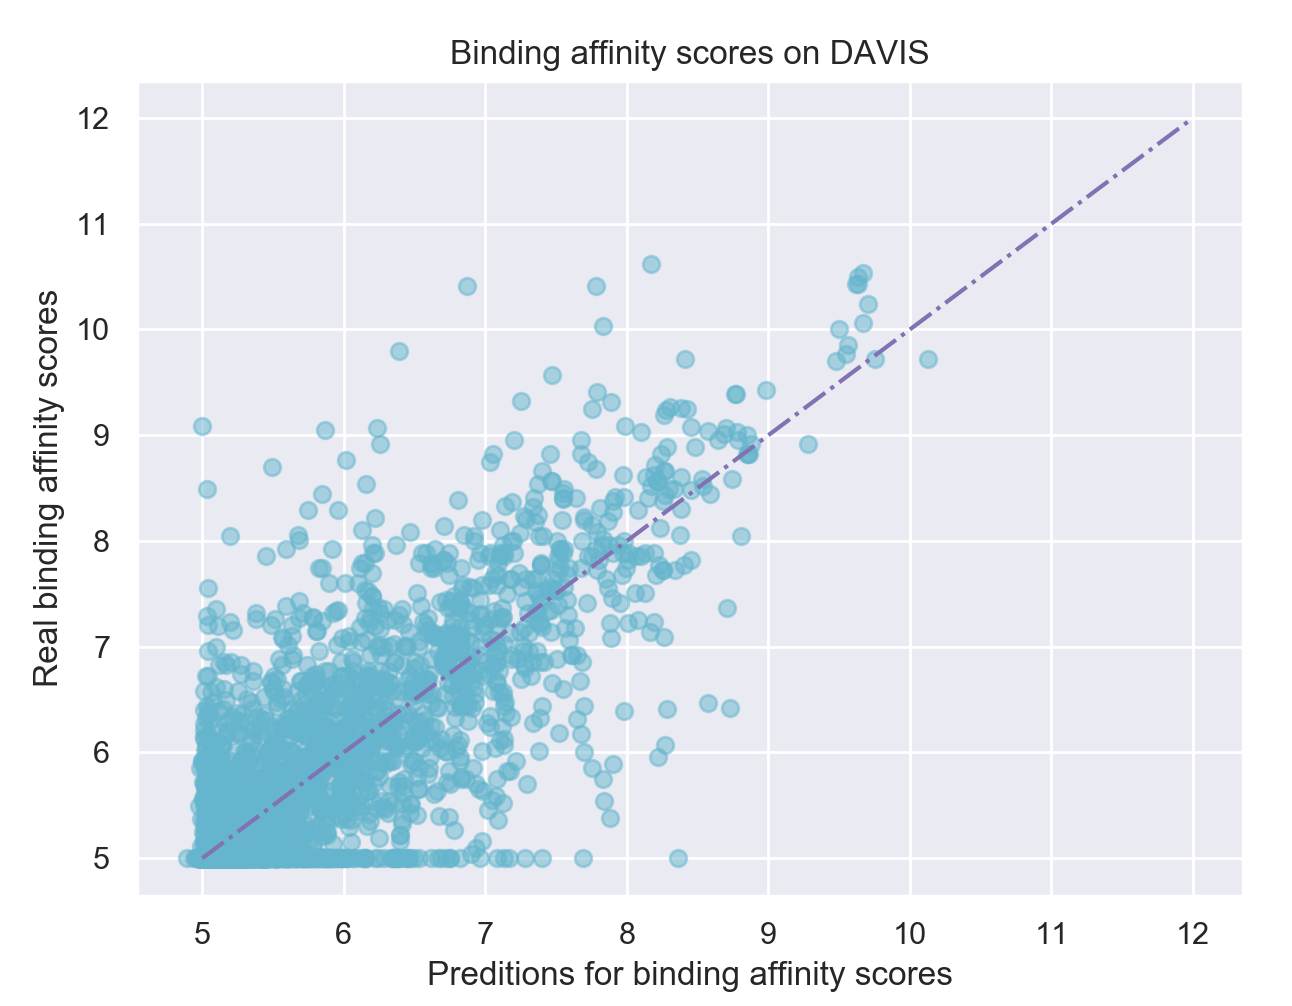
\includegraphics[width=0.85\textwidth]  {imgs/davis-affinity.png}
\bicaption[在 Davis 数据集上,真实分数 VS EmbedDTI 预测分数]{在 Davis 数据集上,真实分数 VS EmbedDTI 预测分数。}
{Predicting scores VS. Real scores on Davis test dataset.}
\label{fig:davis-affinity}
\end{figure}

\subsection{EmbedDTI 在 KIBA 数据集上的表现}

\begin{table}[!htbp]
\centering
\bicaption[EmbedDTI 与基准模型在 Davis 数据集上的比较]{EmbedDTI 与基准模型在 Davis 数据集上的比较}{Comparison of MSE and CI scores on Davis test set}
\begin{tabular}{c|c|c|c|c}
\toprule
模型 & 靶标蛋白的表示 & 药物分子的表示 & MSE & CI \\ 
\midrule
\multicolumn{5}{c}{基准模型} \\
\midrule
KronRLS & Smith-Waterman & Pubchem-Sim & 0.411 & 0.782\\ 
SimBoost & Smith-Waterman & Pubchem-Sim & 0.222 & 0.836 \\
DeepDTA & 1D & 1D & 0.194 & 0.863 \\
WideDTA & 1D+PDM & 1D+LMCS & 0.179 & 0.875\\
GraphDTA\_GCN & 1D & Graph & 0.139 & 0.889 \\
\midrule
\multicolumn{5}{c}{我们提出的模型} \\
\midrule
EmbedDTI\_noPre & 1D & Graph+Graph & 0.134 & 0.896 \\ 
EmbedDTI\_noSub & 1D & Graph & 0.134 & 0.893 \\
EmbedDTI\_noAttn & 1D & Graph+Graph & \textbf{0.131} & \textbf{0.901} \\
EmbedDTI & 1D & Graph+Graph & 0.133 & 0.897 \\ 
\bottomrule
\end{tabular}
\label{table:kiba}
\end{table}

对于 KIBA 数据集,我们将 EmbedDTI 的性能与上一节中描述的同样的基准模型进行了比较。 表 \ref{table:kiba} 显示了他们的 MSE 和 CI 分数。 可以看出,尽管 KIBA 比 Davis 大得多,但这些模型的性能与在 Davis 数据集上的表现趋势相同。 基于原子和子结构的两个药物分子结构图的药物表示学习大大提高了性能,MSE 比 WideDTA 提升了 0.268,比 GraghDTA 提升了 0.058,CI 比 GraphDTA 提高了 0.012。预测分数和真实分数绘制在图\ref{fig:kiba-affinity}中,表明EmbedDTI的预测值接近真实值。

\begin{figure}[!htbp] 
\centering
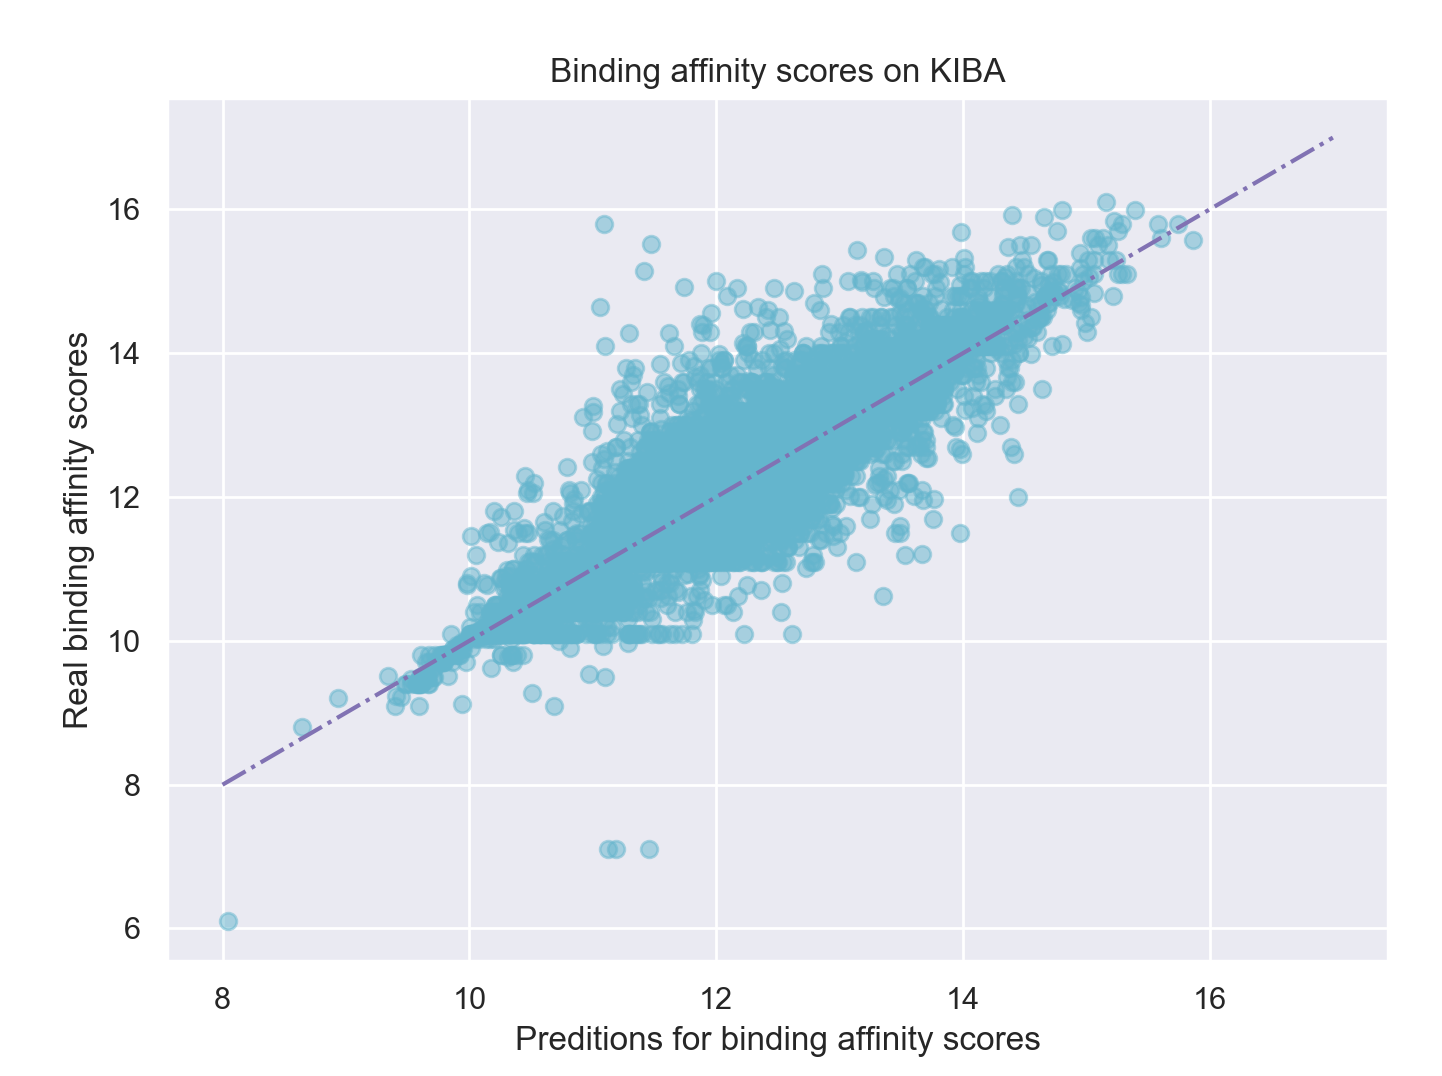
\includegraphics[width=0.85\textwidth]  {imgs/kiba-affinity.png}
\bicaption[在 KIBA 数据集上,真实分数 VS EmbedDTI 预测分数]{在 KIBA 数据集上,真实分数 VS EmbedDTI 预测分数。}
{Predicting scores VS. Real scores on KIBA test dataset.}
\label{fig:kiba-affinity}
\end{figure}

综上所述,在两个数据集上,EmbedDTI 均实现了最低的 MSE 值和最高的 CI 值。特别是,与基线模型的比较表明,靶标蛋白质和药物分子的表征学习都有助于提高模型在 DTI 任务上的性能。

\subsection{EmbedDTI 模型注意力机制的可视化解释}

正如我们在第 \ref{5.2} 节中提到的,GCN 中有一个注意力机制层来学习每个节点(原子或子结构)的重要性。 通过输出每个节点的注意力分数,我们可以观察到 EmbedDTI 模型关注的焦点。

\begin{figure}[!htbp] 
\centering
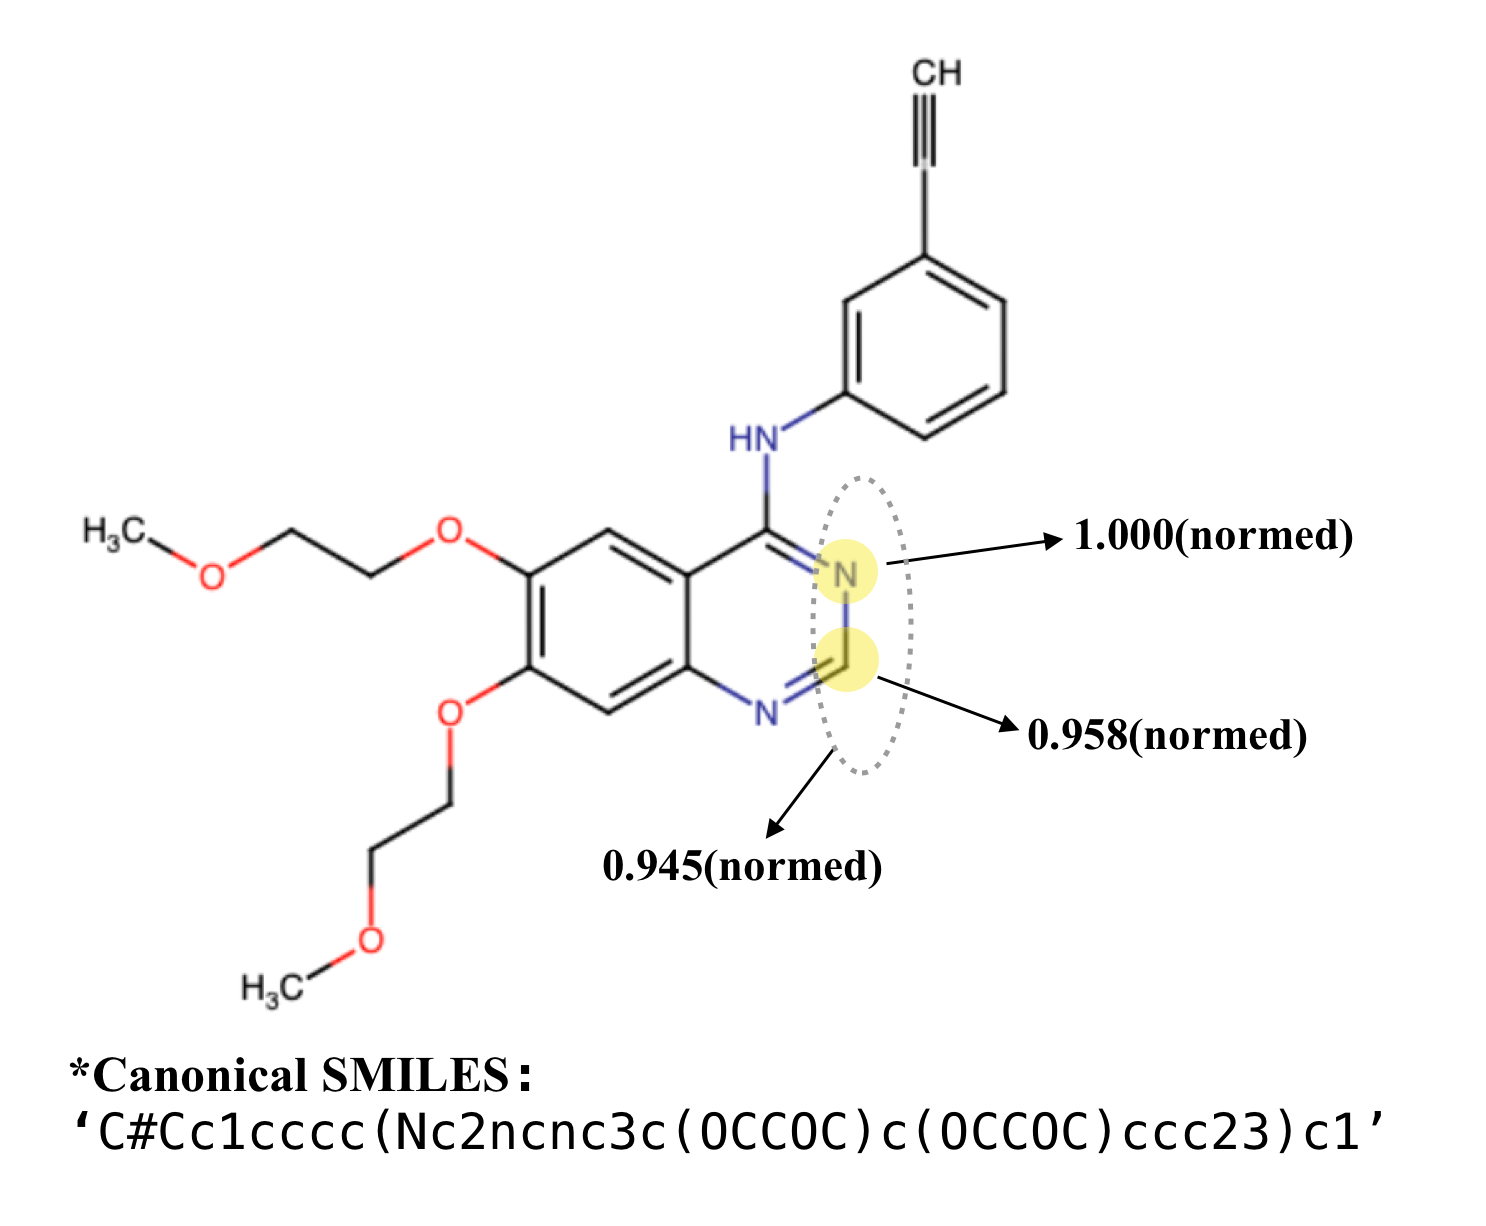
\includegraphics[width=0.7\textwidth]  {imgs/attention.png}
\bicaption[具有$29$个原子和$17$个子结构的稠合氮杂环化合物分子]{具有$29$个原子和$17$个子结构的稠合氮杂环化合物分子。通过注意力输出,图中高亮显示了具有最高归一化注意力分数($1.0$ 和 $0.958$)的两个原子 C(id=13) 和 N(id=14)(我们对分数进行了 min-max 归一化),其中包含两个节点的子结构的注意力得分为 $0.945$。我们预测这些节点在药物-靶标相互作用方面很重要,比如具有潜在的反应活性。}
{A fused nitrogen heterocyclic compound molecule with $29$ atoms and $17$ substructures (processed by partition algorithm). By~attention output, the~two atoms, C(id=13) and N(id=14) with highest normalized attention scores ($1.0$ and $0.958$) are highlighted in the figure (we perform min-max normalization on the scores). The~substructure containing the two nodes is assigned with an attention score of $0.945$.}
\label{fig:att}
\end{figure}

图 \ref{fig:att} 展示了一个示例。图中具有最高注意力分数的两个原子 C (id=13) 和 N (id=14) 被高亮显示,他们分别获得了 1.0 和 0.958 的归一化注意力分数。此外,他们的所属的子结构也获得了 0.945 的高分。

我们注意到,在药物分子结构中,这两个原子所在的位置存在喹唑啉支架。根据 Kamel \cite{kamel2016synthetic}所述,喹唑啉环系统被认为是抗惊厥治疗的“万能钥匙”,因为它构成了许多常见抗惊厥药物的基础支架。事实上,许多带有这种喹唑啉酮支架的结构都会显示出有效的抗惊厥特性,如图 \ref{fig:quinaz} 所示。


\begin{figure}[!htbp] 
\centering
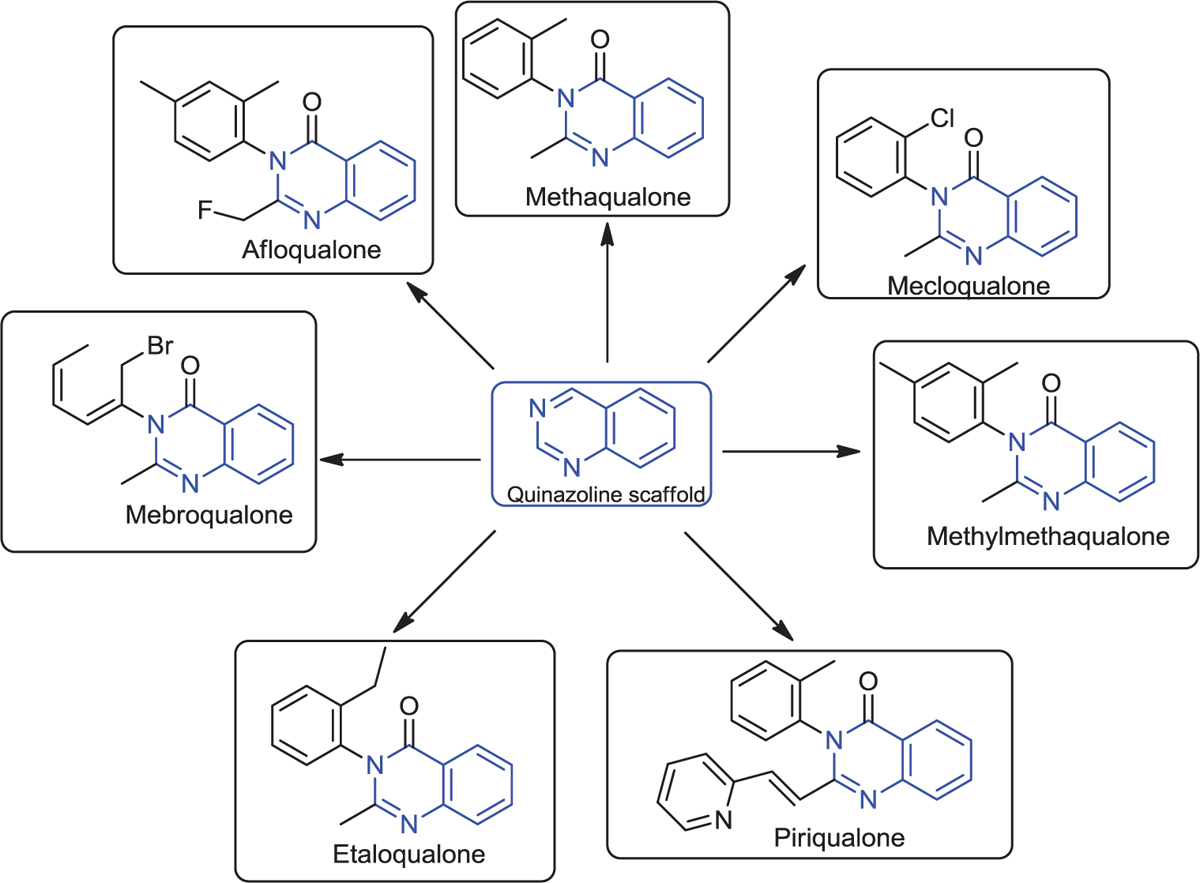
\includegraphics[width=0.85\textwidth]  {imgs/derivatives.jpg}
\bicaption[一些带有喹唑啉酮环的强效抗惊厥药物]{一些带有喹唑啉酮环的强效抗惊厥药物[\cite{kamel2016synthetic}]。}
{Some of the potent anticonvulsant drugs bearing the quinazolinone ring [\cite{kamel2016synthetic}]}
\label{fig:quinaz}
\end{figure}

\section{本章小结}
本章详细介绍了我们提出的基于靶标蛋白质序列和药物分子序列的表征学习的 DTI 预测模型。我们首先介绍了 DTI 任务所需的实验数据集,接着从组成模型的三个部分(初始特征提取、基于深度学习特征训练和结合亲和力预测)详细介绍了模型对靶标蛋白质序列的特征提取和表征学习的方法。同时介绍了对药物分子序列处理为原子级图表示和子结构级图表示的算法和对药物分子结构图进行表征学习的过程。之后,通过对比其他的 DTI 基准模型,验证了我们设计的模型的有效性和优秀的性能同时证明了蛋白质和药物分子序列表征学习的有效性。最后,我们通过一个例子,对我们设计的模型中注意力机制进行了可视化解释。